% Original template ripped from:
% http://www.cs.technion.ac.il/~yogi/Courses/CS-Scientific-Writing/examples/simple/simple.htm


\date{\today}

\documentclass[12pt]{report}

\usepackage{caption}
\usepackage{graphicx}
\usepackage{lmodern}
\usepackage{listings}
\usepackage{idrislang}
\usepackage{amsfonts,amsthm,amsmath}
\usepackage[margin=3.5cm]{geometry}
\usepackage[en,nat,farve,titelside]{ku-forside}
\usepackage[mark,missing={CONFIGURE gitinfo2 PACKAGE}]{gitinfo2}

\renewcommand{\gitMark}{\gitBranch\ :\ \gitHash\ \textbullet{}\ (\gitAuthorDate)\ \textbullet{}\ \gitFirstTagDescribe}

\newtheorem{defn}{Definition}[section]

\opgave{M.Sc. Thesis}
\forfatter{
        Casper Holmgreen and Knut Liest\o l
        % going by alphabetical order here....
}
\title{DPDT: Differential Privacy with Dependent Types}
\undertitel{or: How I Learned to Stop Worrying and Love Dependent Types}
\vejleder{Supervised by Ken Friis Larsen}
\dato{November 11, 2015}


\begin{document}
\maketitle

\lstset{language=idris,
basicstyle=\ttfamily\footnotesize,
frame=single,
numbers=left,
breaklines=true,
postbreak=\raisebox{0ex}[0ex][0ex]{\ensuremath{\color{red}\hookrightarrow\space}}
}

% TODO 1 : add problem statement to introduction
% TODO 1 : improve evaluation by focusing on Hypothesis / Conclusion
% TODO 1 : improve evaluation by comparing # of programs in PINQ vs DPDT

\graphicspath{{assets/}}

\begin{abstract}
With more personal data being stored in the ``cloud'' every day, privacy is becoming an important topic for public discussion.
Private data is potentially quite useful, but cannot be released in its raw form due to privacy concerns.
Differental privacy is an emerging field of research aiming to protect the privacy of individuals participating in a database while maximizing its utility.

PINQ is a framework for the C\# enforcing differential privacy constraints over top of the popular integrated query language, LINQ.
Users are able to build complex, differentially-private queries from a few carefully implemented primitives.
PINQ data providers are then able to dynamically reject queries which could put private information at risk.

Type systems can statically verify programs for varying degrees of correctness.
Dependent types are a particularly powerful feature of certain type systems which lend themselves to tracking differentially privacy metrics.

We implemented a prototype of a differentially-private query language, DPDT, in the dependently-typed, functional programming language Idris.
We outline the benefits and drawbacks we found using dependent types for enforcing differential privacy.

DPDT is loosely modelled on PINQ.
However, whereas PINQ verifies privacy constraints dynamically, DPDT is able to do it statically.
In addition, DPDT is completely type-safe in all of its relational algebra operations.

Limitations of DPDT in comparison to PINQ are backend support, and expressibility in some cases.
However, a large number of side-channel attacks that PINQ is unable to stop are impossible in our language.
\end{abstract}

\clearpage
\tableofcontents
\clearpage
\listoffigures
\clearpage

\chapter{Introduction}\label{sec:introduction}

With each passing day, more and more of our personal information is being collected, cataloged and analyzed by an ever increasing number of interested parties.
Their interests range from selective marketing to collecting business performance metrics and from publicly-funded academic research to unauthorized and potentially illegal surveillance.
We aren't able to curate or control the data they are collecting about us.
In fact, the ubiquity of automatic data collection probably gives them a better picture of you than they would get if you did curate and volunteer the data.
Therefore, as the producers and descriptees of this data, we should be concerned with how it is being used.

There are many creative ways to use data and not all of them align so simply with ``good'' and ``bad''.
Additionally, there is some information that a few trusted people (or systems) must know, but we might not necessarily want our nosy neighbor knowing.
Publicly available data can also help researchers to discover or verify solutions for various societal problems.

Consider Alice's medical records.
Alice's doctor should have access to this very sensitive information, but her neighbor and insurance salesman probably should not.
Recognizing the importance of the right to privacy, some countries have imposed legal privacy requirements on systems maintaining sensitive information, such as medical records (e.g. the Health Insurance Portability and Accountability Act (HIPAA) in USA).
However, Alice's medical records contain valuable data for researchers aiming to understand health trends in our society, but they can't access it without violating her privacy.

Public health researchers would be able to monitor and analyze the long-term health trends of a population over time.
Epidemiologists could detect infectious diseases early and prevent their spread.
The benefits of increased data availability are not limited to public health, either.
Databases containing large amounts of sensitive information can be tremendously valuable for researchers looking into a variety of important questions.

Big data offers us an amazing opportunity for learning about us, but how do we do it without also learning about Alice (as an individual)?
Differential privacy is an active field of research, with input from many different disciplines, that aims to answer this question\cite{journals/cacm/Dwork11}.
The goal of differential privacy is to minimize the risk for the individual while maximizing the utility of the data.

% TODO 1 : add problem statement
% TODO 1 : maybe move contributions up here? or at least outline rest of chap.
This thesis ...

\section{Differential Privacy}\label{sec:intro-diffpriv}

The question of how to provide access to sensitive data is not a new one.
Many techniques for data sharing with privacy constraints have been explored.
They can generally be partitioned into two main approaches: \textit{interactive} (i.e. requires the participation of a ``middle man'') and \textit{non-interactive} (i.e. can be released directly to the public).

One example of a non-interactive approach which has received significant news\footnotemark[\ref{fn:aol}] coverage\footnotemark[\ref{fn:twitter}] a few times\footnotemark[\ref{fn:netflix}] by now\footnotemark[\ref{fn:gic}], is to anonymize or otherwise ``fuzz'' a dataset before releasing it to the public.
However, it is very difficult to release a database that is both useful and private.
Other approaches suffer similar problems relating to privacy or are infeasible to maintain\cite{journals/cacm/Dwork11}.

Differential privacy differentiates itself from other private data release mechanisms by defining privacy differently.
Early approaches often modeled their definition of privacy on the concept of \textit{perfect secrecy} from cryptography: could an adversary with access to the system learn \textit{anything} about an individual?
While this definition is appealing for simplicity, it is too rigid: we actually do want somebody somewhere to learn something.
\footnote{One interesting implication of this is that the adversaries are also the analysts; i.e, we must protect against legitimate users of the system.}
Instead, differential privacy simply offers that Alice's participation in the database can increase her privacy risk by \textit{at most} some negligible amount.

% TODO 1 : add ref to indistinguishability
% Section~\ref{subsec:intro-almostperfectpriv} will expand on this.

\subsection{Indistinguishability}\label{subsec:intro-indistinguishability}

One of the centrals ideas driving differential privacy is that of indistinguishability, i.e. a query evaluated against a dataset should return more-or-less the same result regardless of whether Alice's records were included in the data.
If the result of the query with Alice included is indistinguishable from the result of the query without her, then the contents of Alice's records must be indistinguishable, too.

Indistinguishability is typically achieved by combining the true (distinguishable) result of a query with enough random noise to mask Alice's participation in the database.
However, additive noise is insufficient by itself to guarantee privacy.
An adversarial analyst could simply repeat semantically equivalent queries and average the results.
As the number of evaluated queries approaches infinity, the average will approach the true mean and Alice's personal information is now public.
This susceptibility to averaging repeated queries is one of the major factors preventing non-interactive database anonymization without greatly affecting its utility.

One interactive (and naive) solution is to maintain a query log recording every query ever evaluated against the database.
Incoming queries can then be checked against previous ones to ensure that they can be answered without violating privacy guarantees.
However, two syntactically different queries may be semantically equivalent.
There is no way for a machine to know without running the query and human labor is costly and error-prone.
Additionally, the act of refusing a query could itself be disclosive.

Another (interactive) solution is to limit the number of queries which can be run against the dataset.
However, some queries reveal more information than others, so this seems too crude.
Instead of counting the number of queries, we associate each query with a \textit{privacy cost}.
Then, each dataset is given a \textit{privacy budget}, which limits the total cost of queries that can be run against it.
Each query evaluated reduces the privacy budget by its cost until it is eventually depleted, at which point the data should be destroyed.

\subsection{Almost Perfect Privacy}\label{subsec:intro-almostperfectpriv}

Early privacy research focused on preventing an adversary from learning anything about a particular individual (e.g. Alice).
However, this definition is both impractical and unobtainable.
%impractical because
%unobtainable because
However, this has proven to be nearly impossible in the presence of auxiliary information.
Ganta et al. showed that \textit{k-anonymity} and other proposed partition-based anonymization approaches are vulnerable to composition attacks\cite{ganta2008composition}.
A composition attack is performed on an ``anonymized'' data set by matching it with auxiliary data, such as data from the web, public records, or domain knowledge.
With this technique, an attacker might be able to deduce information about Alice's records in an ``anonymized'' set.

Compositions attacks are not only interesting to academics, either.
AOL\footnote{\label{fn:aol} http://arstechnica.com/business/2006/09/7835/}, Twitter\footnote{\label{fn:twitter}http://arstechnica.com/tech-policy/2009/03/pulling-back-the-curtain-on-anonymous-twitterers/}, Netflix\footnote{\label{fn:netflix}http://arstechnica.com/tech-policy/2009/09/your-secrets-live-online-in-databases-of-ruin/}, and the Massachusetts Group Insurance Commission (GIC) database\footnote{\label{fn:gic}http://web.mit.edu/sem083/www/assignments/reidentification.html} have all suffered publicly in the wakes of linkage attacks.

Rather than trying to prove the impossibility of a privacy breach, differential privacy guarantees that a users participation in a database can only increase their risk of a privacy breach by some negligible amount.
This is true regardless of how much auxiliary information a would-be attacker knows or might learn in the future.

Analysts are able to run differentially private algorithms against private data knowing that no individuals' privacy can be compromised.
Suddenly, many of the Big Data databases which would otherwise be off limits can be made available to researchers.
Each individuals participation in the database has a negligible effect on their risk of a privacy breach, so honest participation follows as a direct consequence.

In fact, a classic example of differentially private thinking is randomized response.
Randomized response is a technique originally proposed in 1965 for encouraging survey respondents to answer potentially embarassing or legally complicated questions honestly\cite{warner1965randomized}.
By introducing an element of randomness, participants are given plausible deniability regardless of how they respond.

After reading the question, participants are instructed to flip a coin.
If the coin yields ``tails,'' the participant responds ``Yes''.
If the coin reads ``heads,'' he/she answers truthfully.
The net result is that $1/2$ of the responses are ``Yes'' by default, while the other half should be a representative sampling of the population.
Thus, if researchers using randomized response find that 70\% of participants admit to an illegal activity, they will know that the true percentage is actually around 40\% and all database participants are given plausible deniability.

\subsection{Algorithms and Metrics}

Many algorithms and metrics have been developed by the differential privacy community.
Each algorithm is typically bundled with some sort of proof that it meets some privacy constraints or has some other privacy-related properties.
The burden of producing such a proof and algorithm is typically manual, and therefore error-prone.

PINQ is a differential privacy framework that takes a different approach\cite{mcsherry2010privacy}.
It is an embedded, SQL-like \textit{domain specific language} (DSL) for the Microsoft .NET languages which guarantees differential privacy by construction.
Users of PINQ are able to compose carefully implemented primitives to build differentially private computations.
The composition of these primitives happens according to well-defined rules, allowing PINQ to track privacy metrics as users build complex differentially private algorithms.
A trusted runtime-system tracks and rejects queries whose cost exceed the remaining privacy budget.

PINQ and its trusted system manage the budget at runtime.
An analyst has no way of knowing whether a query will be accepted without manually tracking their budget.
Reed and Pierce solve this by building a strongly-typed programming language which represents query costs in the types\cite{conf/icfp/ReedP10}.
We aim to build on this idea by demonstrating that a dependent type system is a natural fit for capturing differential privacy requirements.

\section{Dependent Types}\label{sec:intro-deptyps}
% TODO 1 : add more about what dep.typ.s are
% TODO 1 : add problem statement / hypothesis

Strongly-typed programming languages are capable of statically verifying programs for type-correctness, precluding many potential sources of runtime errors: ``well-typed programs can't go wrong''.
We extend this notion of being ``well-typed'' to include differential privacy metrics.
Just as PINQ is embedded in the .NET languages (particularly C\#), our implementation is embedded within the dependently-typed, functional programming language Idris\footnote{http://idris-lang.org}.
This allows us to take advantage of Idris' parser and advanced type-checker, as well as the many improvements continually being made by Idris' active open-source community.

Well-typed programs in our embedded language can't go wrong and also can't violate their privacy requirements.
Formal proofs for type-correct algorithms written in our language are unnecessary - the program itself is the proof.
Thus, all type-correct programs must respect expected privacy constraints.

\section{Contributions}

This paper describes a prototype implementation of an \textit{embedded domain specific language} (EDSL), \texttt{DPDT}, for describing differentially private computations using dependent types.
Originally limited to a handful of academic proof assistants, dependently-typed languages have a come a long way since Per Martin-L\"of presented his intuitionistic type theory (TT)\cite{mlitt}.
General purpose, practical programming languages such as Agda\footnote{http://wiki.portal.chalmers.se/agda/pmwiki.php} and Idris are under active development.
We show that dependent types are a natural fit for describing and verifying differential privacy constraints.

We implemented a fully-typed abstract language for describing the relational algebra; and we developed a simple in-memory Idris database backend for it.
Our main contribution is the layering of differential privacy metrics into the types over top of the fully-typed relational algebra.
PINQ's differential privacy metrics are checked dynamically at runtime, whereas our privacy layer leverages the power of dependent types to verify that privacy constraints are not violated \textit{at compile time}.

\paragraph{Outline}

In Chapter~\ref{sec:differential_privacy}, we cover some necessary background for understanding the basics of differential privacy.
Chapter~\ref{sec:dependent_types_in_idris} serves as a brief tutorial to Idris with a focus on the language features we make use of in our implementation.
Chapter~\ref{sec:function_sensitivity} combines the contents of the previous two chapters in an example implementation of function sensitivity.
Chapter~\ref{sec:RADT} reviews the relational algebra and how we represent it using dependent types.
Chapter~\ref{sec:our_implementation} covers the differential privacy layer that we built over top of the fully-typed relational algebra.
We evaluate our work in Chapter~\ref{sec:evaluation} and provide concluding remarks in Chapter~\ref{sec:conclusion}.

\chapter{Differential Privacy}\label{sec:differential_privacy}

In this chapter, we will focus on specific ideas from the differential privacy literature as it relates to the implementation of our language, DPDT.
In particular, we will discuss function sensitivity, which is a relative measure of how much a function can magnify the distances between collections of objects; and indistinguishability, which is the key idea which quantifies what it means for a computation to be differentially private.
Finally, we describe PINQ, the framework that allows users to build differentially private computations by construction.

\section{Function Sensitivity}\label{subsec:fn_sens}

Function sensitivity is an important concept from the differential privacy literature.
We can make assertions about an entire program if we understand the sensitivities of the functions with which it is composed.
Sensitivity is a key part in making our type system work.

Function sensitivity captures the idea of how relatively ``far'' a function can magnify the distances between pairs of objects.
We say that a function is $c$-sensitive if, for all pairs of inputs, the distance between the outputs does not exceed $c$ times the original distance between the inputs.

\begin{defn}\label{def:csens}
  A function, $f : \mathbb A \rightarrow \mathbb A$, is $c$-sensitive if
  $$\forall x,y.\; d_{\mathbb A}(f(x),f(y)) \le c \times d_{\mathbb A}(x,y)$$
\end{defn}

For a concrete example, let us turn our attention to the domain of real numbers.
We will take the distance function to be the absolute value norm; i.e. $d_\mathbb{R}(x,y) = |x - y|$.
Obviously, the function $f_{id}(x)=x$ cannot magnify distances at all.
For any two real numbers, their difference will equal the difference between them after applying $f_{id}$.

\[
  \forall x,y.\; d_\mathbb{R}(f_{id}(x),f_{id}(y)) = d_\mathbb{R}(x,y)
\]

We say $f_{id}$ is 1-sensitive because distances can't be magnified at all.
Another example of a 1-sensitive function is $f_{1/2}(x) = x/2$; in fact, $f_{1/2}$ is also $\frac{1}{2}$-sensitive.

\begin{defn}\label{def:clessthancprime}
  A function that is $c$-sensitive is also $c'$-sensitive for all $c < c'$.
\end{defn}

Similarly, consider the case where $f_{+10}(x) = x + 10$.
Clearly, it doesn't matter which $x$ and $y$ you sample; the distance $d_{\mathbb R}(x,y)$ will always equal $d_{\mathbb R}(f(x),f(y))$.
Therefore, $f_{+10}$ is a 1-sensitive function.
Now consider the case of $f_{\times 2+10}(x) = 2x + 10$.
Distances between input and output objects can now be doubled (but no more), so it is a 2-sensitive function.
Intuitively, when dealing with linear functions on $\mathbb R$ and the absolute value norm, the largest linear coefficient will dictate the c-sensitivity.
Higher order polynomials are necessarily $\infty$-sensitive.
See Figure~\ref{fig:fn_sens} for a visualization of function sensitivity on $\mathbb R$.

\begin{figure}
    \centering
    \def\svgwidth{\columnwidth}
    \input{assets/RealDistances.pdf_tex}
    \caption{Visualizing function sensitivity on $\mathbb{R}$}
    \label{fig:fn_sens}
\end{figure}

Simple functions on $\mathbb R$ and one dimensional distance functions are not particularly interesting.
However, function sensitivity can be applied much more generally and to much more interesting domains, such as databases containing sensitive information (e.g. Alice's tax records or health information).

We will use $\mathbb D$ to describe the domain of all possible databases.
Hence, a function $f : \mathbb D \rightarrow \mathbb D$ is an endomorphism for databases.
The distance between two databases is their symmetric difference; i.e. $d_{\mathbb D}(D_1,D_2) = | D_1 \ominus D_2 |$.

There is a special case that turns up often in the differential privacy literature.
We are primarily concerned with whether a particular individual's records are included in the database or not, so we often focus on adjacent databases.
We say that two databases are adjacent if they differ by exactly one row.

\begin{defn}
  We denote the case when two databases, $D_1$ and $D_2$, differ by exactly 1 row (i.e. $d_{\mathbb D}(D_1,D_2)=1$) with the special notation: $D_1 \sim D_2$.
  We say that $D_1$ and $D_2$ are adjacent.
\end{defn}

Despite the domain change, function sensitivity behaves exactly as outlined before.
Consider a database endomorphism, $filter_p : \mathbb D \rightarrow \mathbb D$, which filters rows according to some pre-specified predicate, $p$.
$filter_p$ is a 1-sensitive function because it is impossible for it to magnify the distances between databases.

For all pairs of databases, $D_1$ and $D_2$, the distance between them is $d_{in} = d_{\mathbb D}(D_1,D_2)$.
The distance $d_{out} = d_{\mathbb D}(filter_p(D_1),filter_p(D_2))$ cannot exceed $d_{in}$.
$filter_p$ will only remove rows from a database, or leave them unchanged, so we have only to consider the three possible cases of removal.
There are three main cases to consider:
\begin{enumerate}
  \item the filter removes a row that is in both of the databases,
  \item the filter removes a row that is in exactly one of the databases, and
  \item the filter removes a row that is in neither of the databases (does nothing).
\end{enumerate}

\paragraph{Case: the filter removes a row that is in both of the databases.}
Because the row is included in both of the input databases, their symmetric difference is unaffected by its presence.
The row is in neither of the output databases, so their symmetric difference is also unaffected.
Therefore, after the removal of the one row, $d_{out} = d_{in}$.

\paragraph{Case: the filter removes a row that is in exactly one of the databases.}
The symmetric difference of the input databases is affected by this row, because it is in one, but not the other.
Therefore, this row is contributing to the distance between the input databases.
Its removal will bring the output databases closer together.
Therefore, $d_{out} < d_{in}$.

\paragraph{Case: the filter removes a row that is in neither of the databases.}
This is nearly the same as the first case.
The output distance is equal to the input distance: $d_{out} = d_{in}$.

\paragraph{} % to get a blank line between last P and this one
In all cases, $d_{out}$ is either less than or equal to $d_{in}$ after the removal of one row, so we conclude that the removal of any single row will either result in the distance between databases shrinking or remaining unchanged.
Then it follows that the removal of another row isn't going to increase the distance.
Generalizing this to the removal of $n$ rows, we conclude that $d_{out} \le d_{in}$ regardless of how many rows are removed from either database.
Thus, we can fix $c=1$ and conclude that filtering is a 1-sensitive function.

Similar proofs exist for the other relational algebra operators.
Proofs like these provide the basic building blocks used by PINQ and DPDT.
The real power of PINQ and DPDT, however, comes from the ability to freely combine these building blocks without having to manually consider sensitivities.

Consider two functions, $f : \mathbb A \rightarrow \mathbb A$ and $g : \mathbb A \rightarrow \mathbb A$, with sensitivities $c$ and $c'$, respectively.
What is the sensitivity of the function resulting from their composition, $k = f . g$?
Function sensitivities compose multiplicatively; i.e. $k$ is $(c\times c')$-sensitive.
Sensitivity represents the largest factor by which the distances between pairs of objects can be increased, so it follows that the composition of sensitivities is multiplicative.

\section{Indistinguishability}

Indistinguishability is the key idea that distinguishes differential privacy from similar approaches in privacy research.
If an attacker is unable to determine whether Alice's data even exists in the database, he will be unable to determine the contents of her data.
A query is said to be differentially private if it satisfies this property.

We turn to randomness to achieve this kind of behavior.
Consider a randomized function, $f_r : A \rightarrow B$.
Then, for all $x,y \in A$, if the probability of both $f_r(x)$ and $f_r(y)$ being in $S \subseteq B$ is nearly equal, then it is nearly impossible to determine which input was used.

$$ Pr[f_r(x)\in S] \qquad\approx\qquad  Pr[f_r(y)\in S] $$

This is the core idea behind indistinguishability.
The intrinsic randomness of the function prevents an attacker from deducing anything about the input based on the output.
Now consider a randomized query, or mechanism, $\mathcal M : \mathbb D \rightarrow \mathbb R$.
We say that such a query is $\epsilon$-differentially-private if the inclusion of Alice's data increases her privacy risk by at most $e^\epsilon$.

\begin{defn}\label{def:diffpriv}
  A randomized mechanism, $\mathcal{M} : \mathbb D \rightarrow A$, is $\epsilon$-differentially-private if, for all databases $D_1 \sim D_2$, and all $S \in A$,
  $$Pr[\mathcal M(D_1)\in S] \le e^\epsilon \times Pr[\mathcal M(D_2)\in S]$$
\end{defn}

There are a few restrictions on mechanisms in the context of sensitive databases.
Obviously, there are limits to the types of data that queries are allowed to return.
We can't allow entire tables (computed or otherwise) to be returned, because they will potentially contain the sensitive rows we are trying to protect.
Additionally, queries should not be allowed to return data directly from any particular row.

In fact, queries must be restricted to aggregation operations.
This may seem limiting, but in practice is not so.
Certainly, entire classes of queries and algorithms are precluded by this necessity, but the vast majority of statistical research is performed using aggregations over tables, not querying for the information pertaining to particular individuals.

An additional constraint emerges from the previous one: the data type returned by the aggregation must be a semigroup; i.e. it must have an associative binary operator for folding new values into the aggregate.
This is the case because the order in which rows are considered should have no bearing on the resulting value; otherwise, an attacker may be able to learn something about the ordering of individuals.

Aggregations alone, however, are not capable of protecting privacy.
Consider a database consisting of all patients who have ever been treated at the \textit{ABC ABortion Clinic}.
Alice is one of those patients.
Regardless of what Alice's records actually contain, her mere presence in that database could have serious consequences for her private life if the wrong people found out.
Consider the result of the following query: \textit{How many people named Alice are in the database?}
One.
That is a valid aggregation and Alice is now in trouble.

So how could we have saved Alice?
The final requirement is randomness.
When we run an aggregation, we need to randomize the output to satisfy indistinguishability.
If not, an attacker can draft clever aggregations to deduce private information about particular individuals.
Noising a result before returning it gives database participants plausible deniability.
The aggregation function from earlier will no longer be enough to determine whether any records in the database are related to Alice.
See Figure~\ref{fig:indistinguishability} for a visualization of indistinguishability.

\begin{figure}
    \centering
    \def\svgwidth{\columnwidth}
    \input{assets/Indistinguishability.pdf_tex}
    \caption{Visualizing indistinguishability with sample PDFs from a counting query on $D_1$ and $D_2$, where $D_1\sim D_2$}
    \label{fig:indistinguishability}
\end{figure}

The differential privacy community has largely settled on using the Laplace distribution for generating noise.
There are a number of reasons for this, but the main ones concern symmetry and ease of scaling.
The Laplace distribution resembles a symmetric exponential distribution.
Its diversity parameter, or ``width'', scales predictably with $\epsilon$.
In fact, any $c$-sensitive function can be made differentially private easily.

\begin{defn}
Any $c$-sensitive function can be made $\epsilon$-differentially private by adding a value sampled from the Laplace distribution centered on zero with diversity parameter $b=\frac{c}{\epsilon}$.
\end{defn}

Noise sampled from the Laplace distribution scaled according to $b=c/\epsilon$ is sufficient to mask private information while still providing accurate results.

\section{PINQ}\label{sec:pinq}

This section provides a brief overview of PINQ, the framework that originally inspired DPDT.
PINQ is a privacy layer built over top of the .NET integrated query language, LINQ.
It provides carefully implemented, differentially-private primitives and the ability to compose arbitrarily complex algorithms from them without violating differential privacy.
There are two main components to PINQ: transformations and aggregations.
Each PINQ server will keep track of its own privacy budget and reject queries whose costs exceed the remaining budget.
Once a data source's budget has been consumed entirely, it is impossible to query it again through the PINQ interface.

\subsection{Transformations}

LINQ is a query DSL written for the .NET languages allowing users to manipulate data with relational algebra operators directly in the host language.
In LINQ terminology, these operations are called transformations.
Our work includes a fully-typed LINQ-like implementation in Idris (\texttt{Database.PowerOfPi.Idris}).

PINQ's primary contribution is the addition of a privacy layer around the LINQ query language.
The majority of operations available in LINQ have also been made available in PINQ.
However, some transformations cannot be made differentially private and have been modified or removed.
The word ``stability'' is commonly used when discussing a concept similar to function sensitivity in the context of database transformations.

\begin{defn}
A transformation $T$ is $c$-stable if for all pairs of input databases, $A$ and $B$,
$$
  |T(A)\ominus T(B)| \le c \times | A \ominus B |
$$
\end{defn}

Not all transformations from the LINQ API are $c$-stable for finite values of $c$.
In these cases, PINQ provides modified, boundable versions.
As an example, see Section~\ref{subsec:fn_sens} for a proof that the filter transformation (selection) is 1-stable.
Similar proofs exist for all of the other transformations provided by PINQ\cite{conf/sigmod/McSherry09}.

\subsection{Aggregations}

As shown earlier, the only safe way to return data from a sensitive database is to require that it be an aggregation.
PINQ ensures that the only data being released to analysts comes from its carefully implemented aggregation mechanisms.
Each aggregation is proven to be $\epsilon$-differentially private.
$\epsilon$ is an argument provided by the user for fine-tuning the accuracy of the result.
The larger $\epsilon$ is, the more accurate the result will be.
However, the cost of running the aggregation scales directly with $\epsilon$ and is subtracted from the remaining privacy budget.
The total cost of a query is the product of the transformation stability and $\epsilon$.

The simplest of PINQ's aggregation mechanisms is \texttt{noisyCount}, which returns the number of rows described by the given query plus just enough noise to mask the true response.
\texttt{noisyCount} is a 1-stable operation.
Consider two databases which differ by exactly one row, $D_1 \sim D_2$.
Because we know the databases differ by only one row, the distance between the inputs is $d_{in} = d_{\mathbb D}(D_1,D_2)=1$.
From this, we know that the true counts (before adding noise) of the two databases must differ by one; i.e. $d_{out} = d_{\mathbb R}(count(D_1),count(D_2))=1$.
The distances are the same so we can fix $c=1$ and conclude that \texttt{noisyCount} is a 1-sensitive function.
\texttt{noisyCount} is made $\epsilon$-differentially private by adding Laplacian noise scaled according to $b=1/\epsilon$.

Another aggregation mechanism PINQ provides is \texttt{noisyAverage}.
This aggregation adds a unique challenge with regards to function sensitivity.
Let us assume that we have an expression function, $r : \texttt{Row} \rightarrow \mathbb R$.
$r$ yields a numeric value for each row and we want the average value resulting from all of the rows contained in the query.
Let $f : \mathbb D \rightarrow \mathbb R$ be the aggregation function which maps $r$ onto all rows and reduces them to their average (i.e. $f = \texttt{average . map r}$).
What is $f$'s sensitivity?

Consider the pair of databases $D_1 \sim D_2$.
They differ by exactly one row.
How much of an effect can that one differing row have on the distance between the output averages?
It is impossible to say with the information we have now.

Imagine a database, $D_1$, containing the ages of bachelors students at a particular university.
In the United States, their ages will most likely range from 18 to 22.
For illustrative purposes, let us assume that $trueAverage(D_1) = 20$.
Alice, who just turned 40 and is tired of how frequently her private data is accidentally made public, has decided to go back to college to study differential privacy.
How will Alice's participation in the database affect $trueAverage(D_2)$, where $D_2$ is $D_1$ plus her records?

It depends on how many students already attend the college.
Let's say it is a small college of just one prior student.
Alice's participation has brought $trueAverage(D_2) = 30$!
College of 20,000?
$trueAverage(D_2) = 20.000999$.
So is $c=10$ or is $c=0.000999$?
And we had to assume that we already knew Alice's age to even get this far!
In reality, we will have no idea what outlier values $r$ might yield.
We are unable to quantify the effect of that one row on the aggregate.
Thus, we must conclude that $trueAverage$ is $\infty$-sensitive.

PINQ solves this by forcing \texttt{noisyAverage} to clamp values coming from $r$ to the range $[-1,+1]$.
In doing so, PINQ is able to conclude that no row is able to affect the aggregate by more than 2.
Then we can add noise scaled according to $2/\epsilon$.

What if $trueAverage(D) + Lap(2/\epsilon)$ falls outside of $[-1,+1]$?
PINQ solves this by generating new noise values over and over again until the constraint is satisfied.
We improve on this behavior by noting that the Laplace cumulative distribution function (CDF), which is used to sample from the Laplace distribution, is invertible.
We usually use a uniform random variable sampled from the interval $[0,1)$ to draw indiscriminately from the Laplace distribution.
Our implementation computes the subinterval for the uniform random variable that guarantees the constraint will be met; i.e. whereas we normally would sample $x \in X=[0,1)$, we might restrict our uniform variable to $X=[0.33,0.75)$ because we know that the noise generated at these bounds will satisfy the original constraint.

\begin{figure}
    \centering
    \def\svgwidth{\columnwidth}
    \input{assets/LaplaceCDF.pdf_tex}
    \caption{Visualizing constrained sampling from the Laplace distribution (as in \lstinline{noisyAverage})}
\end{figure}

Of course, the decision to clamp values to the interval $[-1,+1]$ will require analysts to pre-process their data.
This will require users to explicitly express their assumptions regarding the range of possible values that $r$ could return.
If we wanted to compute the average age of the college students from before, we might draft a function translating the interval $[18,22]$ to $[-1,+1]$.
Then, if we get a response of $0.5$, we can translate that back to $21$.

\chapter{Dependent Types in Idris}\label{sec:dependent_types_in_idris}

Idris is a general purpose, pure functional programming language with dependent types.
Dependent types allow types to be predicated on values.
This allows developers to describe many aspects of a program in the types which can be mechanically verified by the compiler.

This section serves only as a brief overview to some of Idris' interesting language features.
For a more complete introduction, see the Idris tutorial\footnote{http://docs.idris-lang.org/en/latest/tutorial/index.html}.
We assume a basic familiarity with functional programming languages.
First, we outline the basic capabilities of dependent types with the classic vector example.
Then, we will move on to introduce some of Idris' features which we used in our implementation of DPDT.

The classic dependent types example is the move from traditional \texttt{cons}-lists to vectors.
A vector is a list-like type that is \textit{indexed} by a natural number representing its length; i.e. the type of a vector is determined in part by the number of elements it contains.
Additionally, like lists, vectors are \textit{parameterized} by their element type.
One consequence of this is that \texttt{Vect 3 a} and \texttt{Vect 5 a} are \textit{different} types.

\begin{lstlisting}[caption={Vector Example},label={lst:vector_example}]
||| Represents a vector indexed by its length
data Vect : (length:Nat) -> (itemType:Type) -> Type
\end{lstlisting}

As illustrated in Listing~\ref{lst:vector_example}, types are first class values in Idris.
The type of types is \texttt{Type} and we can directly access and manipulate \texttt{Type}s like any other value.
Without even knowing the underlying data representation of \texttt{Vect}, we can now discuss dependent type signatures of various vector functions.
How should the type signature of \texttt{append} look?
If we append two vectors, with lengths $n$ and $m$, respectively, the resulting vector should have length $n+m$.
See Listing~\ref{lst:vector_ops_example} for an example of this and others.

\begin{lstlisting}[caption={Vector Operations Example},label={lst:vector_ops_example}]
append  : Vect n a -> Vect m a -> Vect (n + m) a
reverse : Vect n a -> Vect n a
take    : (n : Nat) -> Vect (n + m) a -> Vect n a
\end{lstlisting}

Notice how the signature of \texttt{append} clearly describes the input and output types.
Not only is it useful for users to see descriptive type signatures like these, but it helps to prevent many developer errors.
The type-checker will verify that \texttt{append}'s implementation does indeed return a vector of length $n+m$.
Proper use of dependent types can reduce or even eliminate the need for unit testing.

\section{Construction}

\begin{lstlisting}[caption={Nat definition},label={lst:nats_example}]
||| Represents the natural numbers
data Nat = Z | S Nat
\end{lstlisting}

Data types are constructed using a syntax similar to that of Haskell\footnote{https://www.haskell.org/}.
The data type above represents natural numbers recursively.
There are two constructors, \lstinline{Z} and \lstinline{S Nat}.
\lstinline{Z} constructs a zero and \lstinline{S n} constructs the successor of $n$.

\begin{lstlisting}[caption={List and Vect definitions},label={lst:vect_example_def}]
data List : Type -> Type where
  Nil  : List a
  (::) : a -> List a -> List a

data Vect : Nat -> Type -> Type where
  Nil  : Vect Z a
  (::) : a -> Vect k a -> Vect (S k) a
\end{lstlisting}

Listing~\ref{lst:vect_example_def} contains definitions for \texttt{List}s and \texttt{Vect}s.
Notice how the type signature of \texttt{(::)} for \texttt{Vect} builds the length index with the \texttt{S} data constructor from \texttt{Nat}.
The type signature can loosely be interpreted as ``when you add an element to a vector of length k, the resulting type is a vector of length (k+1)''.

\section{Operator sections}

In addition to named functions, Idris has support for anonymous functions.
Anonymous functions, also called lambda abstractions, can be used to provide the implementation of a function on the fly, without having to make a named one.

\begin{lstlisting}[caption={Anonymous functions Example},label={lst:anon_fns}]
-- Anonymous id fn
\x => x

-- Anonymous integer add fn
\x, y => x + y
\end{lstlisting}

Idris also provides constructs for writing anonymous functions more compactly, namely operator sections.
$(*2)$ is a operator section that simply multiplies a numeric value by 2.
It expands to \lstinline{\x => x * 2}, and can be passed into functions and applied to a numeric argument.

\section{Monadic sequencing and do-notation}

In functional programming, a monad is a structure that abstracts computation in some way.
Monads must support two operations: lifting pure elements ``into'' the computation and sequencing two monadic computations.
How these operations are implemented is monad-specific, but the abstraction they provide is powerful.

One example of a monad instance is the state monad.
Pure functional languages don't directly support global state or mutable variables.
However, state can be represented in such languages by threading the state through a series of function calls.
Functions cannot directly modify the state because it is immutable, but they can modify a local copy of it before passing it on to the next function call.

\begin{lstlisting}[caption={Threading state through function calls, no monad},label={lst:state_example}]
||| State holding one integer
data MyState = MkState Int

||| Add an int to the state's int
addToState : Int -> MyState -> MyState
addToState x (MkState st) = MkState (x + st)

namespace Examples

  add15 : MyState -> MyState
  add15 = addToState 5 . addToState 10

  foo : Int
  foo = let MkState i = add15 (MkState 0) in i
  -- foo == 15
\end{lstlisting}

The burden of threading state around is left to the developer.
Monads allow us to abstract unnecessary details like that away, allowing developers to focus on more important things.
Specifically, monad instances are automatically provided with an alternative syntax for writing monadic code called \texttt{do}-notation.
Idris will simply desugar \texttt{do}-notation syntax to regular function calls.

\begin{lstlisting}[caption={Threading state through function calls with do-notation},label={lst:threading_state_do_notation}]
get       : State s s
put       : s -> State s ()
modify    : (s -> s) -> State s ()
evalState : State s a -> s -> a

addToState : Int -> State MyState ()
addToState x = modify (\MkState i => MkState (i + x))

namespace Examples

  add15 : State MyState ()
  add15 = do
    addToState 5
    addToState 10

  foo : Int
  foo = evalState add15 (MkState 0)
  -- foo == 15
\end{lstlisting}

The \texttt{do}-notation allows us to get the state out of the monad context and update it locally before passing it on to the next computation in the sequence.
Idris gives \texttt{do}-notation to any types overloading the \texttt{return} and $(>>=)$ functions.

\section{Implicit arguments and automatic proof search}

Even though Idris' type checker is rather powerful, there are still correct types that can not be validated by the type checker alone.
The \lstinline{head} function on a list is an example of such a type.
\lstinline{head} returns the first element of the list, but what if that list is empty?
\texttt{List}s do not provide type safety for these kinds of operations by themselves.
The Idris type-checker will require a proof that the list is empty.
The type signature of \texttt{head} in Listing~\ref{lst:head_example} shows two arguments: the first is the list and the second is the proof that the list even has a head element.

\begin{lstlisting}[caption={Taking the head of a list},label={lst:head_example}]
head : (xs : List a) -> (isCons xs = True) -> a
head (x :: xs) Refl = x
\end{lstlisting}

Don't worry too much about the proof is constructed for now.
For proofs which are easily machine-checkable, Idris allows us to mark them as implicit arguments.
The compiler will automatically search for and provide the correct proof if possible so the developer doesn't have to.
In the event that it is unable to find a sufficient proof, the compiler will abort compilation with a descriptive error message.

\begin{lstlisting}[caption={Automatic proof derivation},label={lst:auto_proof_example}]
head : (xs : List a) -> { auto p : isCons xs = True } -> a
head (x :: xs) = x
\end{lstlisting}

Implicit arguments are declared using curly braces and the \texttt{auto} keyword.
Alternative proof search methods are available, but are outside the scope of this paper.
The compiler will complain if it is unable to find a proof automatically, requiring one to be manually provided by the developer.

\chapter{Function Sensitivity in Idris}\label{sec:function_sensitivity}

This chapter demonstrate how we use dependent types to model function sensitivity in Idris.

Modelling function sensitivity with dependent types is straight-forward.
Recall that function sensitivity is a metric describing how much a function can amplify the distances between pairs of objects.

$$ \forall x,y.\; d(f(x),f(y)) \le c \times d(x,y) $$

We want to reflect the sensitivity of a function in its type, so we will need to index the type on some numeric value.
To keep the examples in this chapter simple, we will use \texttt{Float} to represent sensitivity, but our implementation actually uses an implementation of \texttt{Rational}s similar to that in Haskell's \texttt{Data.Ratio}.

Listing~\ref{lst:rep_sens_fns} defines a type constructor indexed by the sensitivity and parameterized by its input and output types.
It has just one data constructor which is used for wrapping native Idris functions.
A \texttt{SensitiveFunction s a b} is a function with sensitivity \texttt{s} mapping from \texttt{a} to \texttt{b}.

\begin{lstlisting}[caption={Representing sensitive functions},label={lst:rep_sens_fns}]
||| Represents a sensitive function
||| @ c The sensitivity of the function
||| @ a The input type of the function
||| @ b The output type of the function
data SensitiveFunction : (c:Float) -> (a:Type) -> (b:Type) -> Type where
    MkSensitiveFunction : (a -> b) -> SensitiveFunction s a b

namespace Examples

    add10 : SensitiveFunction 1 Float Float
    add10 = MkSensitiveFunction (+10)

    doubleThenAdd10 : SensitiveFunction 2 Float Float
    doubleThenAdd10 = MkSensitiveFunction (*2)

    cheat : SensitiveFunction 1 Float Float
    cheat = MkSensitiveFunction (*20)
\end{lstlisting}

Notice the \texttt{cheat} example above.
It is possible to define sensitive functions which intentionally misrepresent their sensitivities.
Our focus here is not on the verification of a function's sensitivity, but rather on the interaction between sensitivity and the type system under operations such as function composition or application.
Unrestricted application is as simple as unwrapping the function and applying it to an argument.
Function composition returns a new type indexed by the combined sensitivies of the underlying functions.
This is done simply by wrapping the composed functions in a new data constructor and letting the types work out the rest.
See Listing~\ref{lst:sens_fns_ops}.

\begin{lstlisting}[caption={Sensitive function operations},label={lst:sens_fns_ops}]
||| Applies a sensitive function to an input
||| @ f The sensitive function to be applied
||| @ x The input
apply : (f:SensitiveFunction s a b) -> (x:a) -> b
apply (MkSensitiveFunction f) x = f x

||| Composes two sensitive functions
||| @ g The outer function
||| @ f The inner function
(.) : (g:SensitiveFunction s b c) -> (f:SensitiveFunction s' a b) -> SensitiveFunction (s*s') a c
(.) (MkSensitiveFunction g) (MkSensitiveFunction f) = MkSensitiveFunction (g . f)
\end{lstlisting}

Now we are able to compose sensitive functions and Idris' type-checker will understand the resulting sensitivities.
See Listing~\ref{lst:composition_examples} for examples of how the type-checker verifies sensitivities.

\begin{lstlisting}[caption={Examples of Sensitive Function Composition},label={lst:composition_examples}]
doSomeMath : SensitiveFunction 2 Float Float
doSomeMath = add10 . doubleThenAdd10

--doesNotCompile : SensitiveFunction 4 Float Float
--doesNotCompile = add10 . doubleThenAdd10

doSomeMath2 : SensitiveFunction ?sens Float Float
doSomeMath2 = add10 . doubleThenAdd10
\end{lstlisting}

One unfortunate consequence of having such a powerful type-system is that all top-level names must have an associated type declaration.
This means that despite the fact that the type-system is capable of computing the costs, we must still explicitly provide the function sensitivity in the type declaration (as in the \texttt{doSomeMath} signature above).
Because the computation is decidable, users will be able to ask Idris for help through its interactive proof search feature.
Asking Idris to find a proof of the hole \texttt{?sens} yields \texttt{fromInteger 2}.

Listing~\ref{lst:sens_app} demonstrates an alternative application function for sensitive functions.
This one checks whether a function's sensitivity exceeds the provided value.
However, this check occurs \textit{at compile time}, not dynamically.

\begin{lstlisting}[caption={Sensitivity-aware function application},label={lst:sens_app}]
||| Applies a sensitive function to an input, if its sensitivity does not exceed z
||| @ z The max sensitivity allowed
||| @ f The sensitive function to be applied
||| @ x The input
applyIfLT : (z:Float) -> (f:SensitiveFunction s a b) -> (x:a) -> { auto p : So (s < z) } -> b
applyIfLT _ f x = f x

namespace Examples

    compiles : Float
    compiles = applyIfLT 2 add10 0

    -- doesNotCompile : Float
    -- doesNotCompile = applyIfLT 2 (doubleThenAdd10 . doubleThenAdd10) 0
\end{lstlisting}

\chapter{RADT - Typing the Relational Algebra}\label{sec:RADT}

In this chapter, we review the relational algebra and show how it can be modelled in a dependently typed language.
We first introduce the relational algebra, after which we describe the implementation of our type-safe relational algebra, RADT (Relational Algebra with Dependent Types).
Our approach is based on Chapter 4 from \textit{The Power of Pi}\cite{OurySwierstra08PowerOfPi}, an excellent resource for practical examples of what dependent types are capable of.

The relational algebra describes semantics for modelling and querying data in relational databases (e.g. MySQL\footnote{https://www.mysql.com/}).
E.F. Codd described relational databases and their associated algebra back in the 1970's\cite{codd70}.
The relational model quickly became popular for its simplicity and good performance.

Tables are the fundamental objects which relations build on.
The rows of a table represent individual entities and the columns represent their attributes.
Each of these columns is associated with a data type.
Every table has a \textit{schema}, which is a list of its column names and their types.
For example, the Table~\ref{tab:people_table} contains four columns; each has a unique name and an associated data type.

\begin{table}[tb]
    \caption{People Table}
    \label{tab:people_table}
    \centering

    \begin{tabular}{|c|c|c|c|}
    \hline

    \hline
    \textbf{Key} & \textbf{Name} & \textbf{Age} & \textbf{FavoriteFood} \\
    \hline
    \textit{Int} & \textit{String} & \textit{Int} & \textit{String} \\
    \hline
    \hline
       1 & Casper & 26 & Rogan Josh Curry \\
       2 & Knut & 26 & Moussaka \\
    \hline

    \end{tabular}
\end{table}

The relational algebra allows us to build structured queries against relational databases.
The primary operators are listed below.
Note that some of the operators may require expressions to be provided (e.g. for filtering a table with a conditional).

\begin{itemize}
    \item selection
    \item projection
    \item Cartesian product\footnote{\label{fn:set_ops} These operations function identically to their set counterparts, but impose additional requirements regarding table schemas. In particular, union and difference (and therefore intersection) require that the schemas of the two operands match. The Cartesian product operator requires that the two schemas are disjoint.}
    \item set union\footnotemark[\ref{fn:set_ops}]
    \item set difference\footnotemark[\ref{fn:set_ops}]
\end{itemize}

Note that the set operations and Cartesian product impose additional requirements in this context.
These extra constraints have precluded many type systems from being able to fully type-check the relational algebra.
Strongly-typed languages, such as Haskell, have devised clever solutions to this problem, but none are as straight-forward as the approach available to a dependent type system.
The ability to capture schemas directly in the types and to manipulate them yields a deceptively simple, but powerful typing framework for relational databases.

\section{Relational Algebra in Idris}

This section will outline the implementation of RADT, our relational algebra EDSL in Idris. 
We begin by defining some simple algebraic datatypes (ADTs) for keeping the types clear.
We then define a toy expression language before moving on to the query language.

First, we need to be able to represent table attributes (columns).
An \texttt{Attribute} is just the pairing of a name (\texttt{String}) to a data type.
Following David Christiansen's lead, we opt to use \texttt{(:::)} instead of the more traditional \texttt{(,)} for constructing our pairs\cite{ChristiansenTypeProviders}.
We believe this enhances readability of long \texttt{Schema}s, which are just lists of \texttt{Attribute}s.

\begin{lstlisting}[caption={Representing attributes and schemas},label={lst:attrs_and_schemas}]
||| Represents an attribute
data Attribute : Type where
  (:::) : String -> Type -> Attribute

||| Represents a schema
Schema : Type
Schema = List Attribute

namespace Examples

    people : Schema
    people = [ "Key"          ::: Int
             , "Name"         ::: String
             , "Age"          ::: Int
             , "FavoriteFood" ::: String
             ]
\end{lstlisting}

The relational algebra assumes the existence of an expression language, so we implement a primitive one for demonstration.
An expression has access to all of a row's attributes during evaluation and can return a value of any type.
So we index expression types by their \texttt{Schema} and parameterize them by the return type.
Thus, an expression with the type \texttt{Expr s a} can be read as an expression with access to the attributes in schema \texttt{s} returning type \texttt{a}.
Notice that we have not yet defined any underlying representation for the rows.

Expressions are built up from other expressions, forming an expression tree.
See Figure~\ref{fig:expr_tree} for an example of a simple singly-typed expression tree.

\begin{figure}[h!]
    \centering
    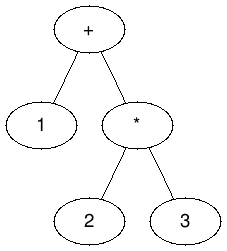
\includegraphics[width=0.25\linewidth]{assets/expr_tree.png}
    \caption{Visualizing expression trees with an example of a simple integer arithmetic expression $(1 + 2 \times 3)$}
    \label{fig:expr_tree}
\end{figure}

% TODO 2 : make a figure of a Query tree showing the types

The return type of the tree in Figure~\ref{fig:expr_tree} is obvious, but what type will a more complex tree from our expression langage have?
Expressions cannot change the schema, so that must remain constant even as the tree grows.
The root of the tree represents the last ``operation'' to be evaluated.
The value returned by this node will be returned, therefore the return type of the root of the tree is the return type of the entire tree.
The type-checker is capable of verifying the types throughout the entire tree, so only well-typed expressions are allowed by the type-system.

\begin{lstlisting}[caption={Representing expressions},label={lst:expressions}]
||| Represents an abstract expression indexed by its schema
||| @ s The schema available to the expression
||| @ a The return type of the expression
data Expr : (s:Schema) -> (a:Type) -> Type where
  ||| Represents a literal value
  Lit    : t -> Expr s t
  ||| Look up a value in the schema
  (^)    : (s:Schema) -> (nm:String) -> { auto p : (map cast s) `ContainsKey` nm } -> Expr s (lookupType s p)
  ||| Represents addition
  (+)    : Num t => Expr s t -> Expr s t -> Expr s t
  ||| Represents equality check
  (==)   : Eq t  => Expr s t -> Expr s t -> Expr s Bool
  ||| Lifts a pure Idris function into the expression language
  PureFn : (a -> b) -> Expr s a -> Expr s b

namespace Examples

  fountain_of_youth : Expr people Int
  fountain_of_youth = people^"Age" - 10

  -- doesNotCompile : Expr people Int
  -- doesNotCompile = people^"Does Not Exist"
\end{lstlisting}

In fact, the type-system is even aware when we try to reference columns that don't exist.
Remember, we haven't even mentioned a backend yet; all of this safety is coming exclusively from the type-system.

One of PINQ's neat features is that users have access to nearly all of the features of the host language.
The \texttt{PureFn} data constructor lifts pure Idris functions into the expression language, which should allow clever developers to bend even this simple expression language into something quite powerful.
This functionality is only available to the Idris backend.

\texttt{ContainsKey} is a proof that the given schema contains the attribute in question.
It is derived automatically, so users of our language should never have to worry about it.
\texttt{lookupType} is able to use this proof to statically verify the types.

The core of the relational algebra consists of the query operators, which we model as follows.
\texttt{Query} is implemented as a data family, allowing us to adjust its internal data representation just enough to implement a variety of backends.
In particular, the representation of tables is backend specific.
For example, an in-memory Idris backend might store pointers directly to the tables in memory, whereas a SQL backend might just store the name of the table as a string.
One of the benefits of this is that any dataset which can be modelled using the relational algebra is usable.

\begin{lstlisting}[caption={Representing queries},label={lst:queries}]
mutual -- required for mutual definitions

  ||| Represents an abstract query
  ||| @ t A function yielding a base table representation given a schema
  ||| @ s The schema of the query
  data Query : (t:Schema -> Type) -> (s:Schema) -> Type where
    Table   :       t s -> Query t s
    Union   : Query t s -> Query t s -> Query t s
    Diff    : Query t s -> Query t s -> Query t s
    Product : Query t s -> Query t s' -> { auto p : Disjoint s s' } -> Query t (s ++ s')
    Projection : (f:String -> Maybe String) -> Query t s -> Query t (projectedSchema f s)
    Select  : Expr s Bool -> Query t s -> Query t s

  ||| Represents an abstract grouping
  ||| @ t A function yielding a base table representation given a schema
  ||| @ s The schema of the query
  ||| @ k The type of the grouping key
  data Grouping : (t:Schema -> Type) -> (s:Schema) -> (k:Type) -> Type where
    GroupBy : Eq k => Expr s k -> Query t s -> Grouping t s k

  ||| Represents an abstract partitioning
  ||| @ t A function yielding a base table representation given a schema
  ||| @ s The schema of the query
  ||| @ k The type of the partitioning key
  data Partitioning : (t:Schema -> Type) -> (s:Schema) -> (k:Type) -> Type where
    Partition : Eq k => List k -> Expr s k -> Query t s -> Partitioning t s k

namespace Examples

  -- Tables in our Idris backend are: List (Row s)
  IdrisBackend : Schema -> Type
  IdrisBackend s = List (Row s)

  -- Tables in our SQLite backend are represented by their names
  SQLiteBackend : Schema -> Type
  SQLiteBackend _ = String
\end{lstlisting}

Recall that the set operators require additional constraints that less powerful type systems have a difficult time capturing.
Set union and difference require that the two operands share matching schemas.
Cartesian product requires that they be disjoint.
Notice how type unification allows us to specify the first two constraints.
The disjoint proof is only slightly more complex; but because it is decidable it can be automatically derived, so the users will be unaware of any additional complexity.

In trying to emulate PINQ, we chose to focus most of our efforts on implementing an in-memory Idris backend.
However, any backend which can be modelled with the relational algebra can be supported and queried in a differentially-private manner.
The exception to this is the \texttt{PureFn} feature, which is only available to Idris-based backends (e.g. an Idris-based server a la LINQ providers).
However, most uses of \texttt{PureFn} could be replaced by extensions to the expression language.

There are two main components required to make a functioning backend implementation:
1) an underlying data representation and
2) evaluator functions that understand our abstract expression and query trees.
Existing database systems such as \texttt{MySQL}\footnote{https://www.mysql.com/} and \texttt{SQLite}\footnote{https://sqlite.org/} already have their underlying data representations.
Implementing backends for them would likely require compiling abstract syntax trees down to SQL strings which could then be submitted to the database.

Our Idris backend uses a basic \texttt{cons}-list structure indexed over \texttt{Schema}s.
Listing~\ref{lst:idris_backend} shows this.
It also shows snippets from expression and query evaluation functions written for Idris and SQLite backends, respectively.

\begin{lstlisting}[caption={Implementing backends (snippets)},label={lst:idris_backend}]
||| Represents a row of data in memory
||| @ s The row's schema
data Row : (s:Schema) -> Type where
  Nil  : Row []
  (::) : Eq t => t -> Row s -> Row (name:::t::s)

namespace IdrisBackend
  ||| Evaluates an abstract expression in the Idris backend
  evalE : Expr s t -> Row s -> t
  evalE (x + y) r = eval x r + eval y r
    [..]

  ||| Evaluates an abstract query in the Idris backend
  evalQ : (q:Query Table s) -> Table s
  evalQ (Product x y) = [ x' ++ y' | x' <- eval x, y' <- eval y ]
    [..]

namespace SQLiteBackend
  ||| Compiles an abstract expression to a SQLite string
  evalE : Expr s t -> String
  evalE (x + y) = "(" ++ eval x ++ ") + ("  ++ eval y ++ ")"
    [..]

  ||| Compiles an abstract query to a SQLite string
  evalQ : Query SQLiteTable s -> String
  evalQ (Product x y)    = "(" ++ eval x ++ ") , (" ++ eval y ++ ")"
    [..]
\end{lstlisting}


\chapter{DPQ - Differentially Private Queries}\label{sec:DPQ}

In this chapter we describe how we bring together the material of the previous chapters and outline the implementation of DPQ.
DPQ is an abbreviation for Differentially Private Queries and is a language for compiling differentially private string queries for query languages. 

The language is built as a layer on top of our relational algebra, RADT, described in the previous chapter.
Our goal is to leverage the Idris type-checker to statically verify differential privacy constraints in single queries.

\section{Transformations}

The first building block in the formation of DPQ was to add the stability metric to RADT's relational algebra operations, or transformations as they are refered to in the differential privacy literature.

New types are created to capture the necessities as shown in Listing \ref{lst:pinqueries}.
Notice that the types are similar to the ones in RADT.
They are now also indexed by a \texttt{Stability} (type synonym for \texttt{Rational}) to capture the stability of a query.
As Idris supports name overloading we have decided to keep the names the same as in RADT.
To avoid confusion these type names will be prefixed with their respective language name throughout this report (e.g., \texttt{RADT.Query}, \texttt{DPQ.Query}).
It should be pointed out that DPQ and DPDT, described in the next chapter, share these data types.
Therefore, both \texttt{DPQ.Query} and \texttt{DPDT.Query} refer to \texttt{Query} from Listing \ref{lst:pinqueries}.

\begin{lstlisting}[caption={Representing privacy-aware queries},label={lst:pinqueries}]
||| Represents an abstract, stability-aware query
||| @ t A function yielding a base table representation given a schema
||| @ s The schema of the query
||| @ c The stability of the query
data Query : (t:Schema -> Type) -> (s:Schema) -> (c:Stability) -> Type where
    MkQuery : Query t s -> Query t s c

||| Represents an abstract, stability-aware grouping
||| @ t A function yielding a base table representation given a schema
||| @ s The schema of the query
||| @ k The type of the grouping key
||| @ c The stability of the query
data Grouping : (t:Schema -> Type) -> (s:Schema) -> (k:Type) -> (c:Stability) -> Type where
    MkGrouping : Grouping t s k -> Grouping t s k c

||| Represents an abstract, stability-aware partitioning
||| @ t A function yielding a base table representation given a schema
||| @ s The schema of the query
||| @ k The type of the partitioning key
||| @ c The stability of the query
data Partitioning : (t:Schema -> Type) -> (s:Schema) -> (k:Type) -> (c:Stability) -> Type where
    MkPartitioning : Partitioning t s k -> Partitioning t s k c
\end{lstlisting}

We will focus on \texttt{DPQ.Query} because \texttt{DPQ.Grouping} and \texttt{DPQ.Partitioning} have similar implementations, but are case-specific.
A \texttt{DPQ.Query t s c} describes a \texttt{c}-differentially private query with schema \texttt{s} (and backend table representation \texttt{(t s)}).
There is only one data constructor which serves simply to wrap a \texttt{RADT.Query}.
This allows us to define a \texttt{RADT.Query} and assign it an arbitrary stability.

Next, we provide the standard operators from the relational algebra as functions operating on \texttt{DPQ.Query t s c}.
We simply unwrap the \texttt{RADT.Query} and then rewrap it in the same \texttt{DPQ.Query} data constructor, but using a different type constructor.
This is because the schema and stability could potentially change.
We control the \textit{application programming interface} (API) that is exported, so we carefully implement the relational algebra operators with the correct stability costs.
By unwrapping and rewrapping the \texttt{RADT.Query} trees from Chapter~\ref{sec:RADT} in our new type, we are now able to build query trees that carry privacy metrics in the type.

\begin{lstlisting}[caption={Representing privacy-aware transformations},label={lst:transformations}]
||| Represents stability-aware selection
where' : Query b s c -> Expr s Bool -> Query b s c
where' (MkQuery q) e = MkQuery (Select e q)

||| Represents stability-aware projection
select : Query b s c -> (f:String -> Maybe  String) -> Query b (projectedSchema f s) c
select (MkQuery q) f = MkQuery (Projection f q)

||| Represents stability-aware union
union : Query b s c -> Query b s c' -> Query b s (c + c')
union (MkQuery q) (MkQuery q') = MkQuery (Union q q')

||| Represents stability-aware intersection
intersect : Query b s c -> Query b s c' -> Query b s (c + c')
intersect (MkQuery q) (MkQuery q') = MkQuery (Diff q q')

||| Represents stability-aware grouping
groupBy : Eq k => Expr s k -> Query b s c -> Grouping b s k (c * 2)
groupBy e (MkQuery q) = MkGrouping (GroupBy e q)
\end{lstlisting}

Recall from Section~\ref{subsec:fn_sens} that \texttt{where'} is a 1-sensitive function.
Notice how its type declaration reflects that.
The \texttt{c} parameter remains unchanged through the rewrapping.

\texttt{union}, however, costs the sum of the costs of the operands.
Notice how this can be precisely specified in Idris.

Of course, we can't just return the results of any query.
A query might just return the database contents untouched, potentially violating every single participant's privacy.
Differential privacy requires that any query response be the result of some sort of aggregation.

\section{Aggregations}



\chapter{DPDT - Differentially Private Programs}\label{sec:DPDT}

Additionally, the control flow of a program may be predicated on the value returned from an aggregation.
Sequential queries are additive in cost.
Sequencing computations in functional programming is traditionally accomplished using the infamous \texttt{Monad}.
In many languages, Idris included, types implementing \texttt{Monad} instances have access to special syntactic sugar, commonly known as \texttt{do}-notation.
\texttt{do}-notation is not magic: it just allows developers to use an alternative syntax for writing monadic code.

We want to take advantage of this, but the type signatures required to satisfy a monad instance preclude our ability to reflect sensitivities in the types.
Fortunately, Idris does not actually require a \texttt{Monad} instance to overload \texttt{do}-notation.
We just need to provide the functions \texttt{$(>>=)$} and \texttt{return}.

\begin{lstlisting}[caption={Representing differentially private mechanisms},label={lst:mechanisms}]
||| Represents a differentially private computation
||| @ c The privacy cost of the computation
||| @ a The return type of the computation
data Private : (c:Sensitivity) -> (a:Type) -> Type
    MkPrivate : (CrapGen -> (a,CrapGen)) -> Private budget a

||| Lifts a value into a private computation
return : a -> Private 0 a
return x = MkPrivate $ \s => (x,s)

||| Sequences two private computations
(>>=) : Private s a -> (a -> Private s' b) -> Private (s + s') b
(>>=) (MkPrivate sf) f = MkPrivate $ \st => let (x,st1)       = sf st
                                                MkPrivate sf' = f x
                                             in sf' st1

||| Evaluates a private computation
evalPrivate : Private s a -> CrapGen -> a
evalPrivate (MkPrivate f) g = fst (f g)

namespace Examples

    nestedAggregations : Private 3 Double
    nestedAggregations = do x <- the (Private 1 Double) someAggregation
                            y <- the (Private 2 Double) someOtherAggr
                            return ((x+y*2)/3)
\end{lstlisting}

Experienced functional programmers will probably recognize that \texttt{Private} is functionally equivalent to a \texttt{State} monad instance.
Laplace noise requires pseudorandom number generation, so we are keeping track of a generator throughout the computation.

Each aggregation is responsible for providing differential privacy.
Our implementation currently provides two common aggregations, \texttt{noisyCount} and \texttt{noisyAverage}.
Experts will be able to write their own aggregations to provide to the public.

Of course, aggregations alone are not sufficient for guaranteeing privacy.
We must add Laplace noise according to the sensitivity of the \texttt{PINQuery} and a user-provided epsilon.

\texttt{noisyCount} is a good example of a simple aggregation.
The user provides a \texttt{PINQuery} (which has an associated stability cost) and an arbitrary epsilon reflecting how accurate they want the result to be.
The added noise is scaled according to the user provided epsilon while the privacy cost of the entire computation is computed in the types.

\begin{lstlisting}[caption={Representing aggregations},label={lst:aggregations}]
||| Differentially private mechanism for counting the
||| number of rows described by a query for the Idris backend
||| @ q The query
||| @ e User provided epsilon, accuracy parameter
noisyCount : (q:PINQuery IdrisTable s c) -> (e:Epsilon) -> Private (c*e) Double
noisyCount (MkPINQuery q) eps = MkPrivate $ \g =>
  let (rx,g') = rndDouble g
      noise   = samplePure 0 (1 / toFloat eps) rx
      count   = the Double $ fromInteger $ fromNat $ length (eval q)
   in (count + noise, g')
\end{lstlisting}

\chapter{Evaluation}\label{sec:evaluation}

In this chapter, we will evaluate how well dependent types allow differential privacy metrics to be tracked and verified in the type system.
We begin our evaluation of DPDT with simple queries before moving on to more complex algorithms.

\section{Differentially private queries}

We begin by verifying the behavior of DPDT with simple queries.
There are enough moving parts in a differentially private mechanism to warrant this.
% TODO 1 : "tell what you want to show"
Listing~\ref{lst:example_data_people} constructs a small database in our Idris backend.

\begin{lstlisting}[caption={Validation Data},label={lst:example_data_people}]
import Database.PowerOfPi.Idris

Person : Schema
Person = [ "Name" ::: String , "Age" ::: Double ]

people : PINQuery IdrisTable Person 1
people = MkPINQuery $ Table [ [ "Alice"  , 40 ]
                            , [ "Casper" , 26 ]
                            , [ "Knut"   , 26 ]
                            , [ "Tor"    , 26 ]
                            , [ "Gismo"  ,  2 ]
                            ]
\end{lstlisting}

Let us consider some primitive queries and their responses.
First, we will try to determine whether Alice's records are included in the database.
This simple example demonstrates several components of our implementation: the expression language, a transformation, and a differentially private mechanism: \texttt{noisyCount}.

\begin{lstlisting}[caption={Counting Alices},label={lst:counting_alices}]
countAlices : Private 1 Double
countAlices = do let isAlice = Person^"Name" == Lit "Alice"
                 let alices  = people `where'` isAlice
                 noisyCount alices 1

testCountAlices : IO Double
testCountAlices = evalPrivateIO alices
\end{lstlisting}

\texttt{isAlice} is an \texttt{Expr Person Bool} for finding those rows which contain ``Alice'' in the name column.
\texttt{alices} is a \texttt{PINQuery IdrisTable Person 1}, because \texttt{where'} has a stability of 1.
It abstractly represents the table of participants named ``Alice''.
Finally, when we invoke the \texttt{noisyCount} mechanism, the Idris backend evaluates the query, computes the desired result and adds noise to it before returning it.

Note that we have chosen to use $\epsilon = 1$ when invoking \texttt{noisyCount} and \texttt{where'} has a stability cost of 1.
Therefore, the cost of the entire computation is 1.

Every time we run \texttt{testCountAlices}, we will get a different response because of the Laplacian noise being added to the result.
Given the \texttt{people} table from Listing~\ref{lst:example_data_people}, we can describe from the outset what we expect the distribution of this query to look like (assuming an infinite budget).
Figure~\ref{fig:indistinguishability} shows the PDF curves for \texttt{countAlices} being run on a database with and a database without Alice.
Given a single value sampled from either of those two PDFs, an analyst will have no way of telling which PDF it came from.

Of course, the analyst could try to sample multiple times, averaging the results, to learn the true mean.
DPDT allows this, but the type system ensures that the cost of the query increases accordingly.
Listing~\ref{lst:nested_aggrs} contains an example of how a malicious analyst might try to average a few queries.

\begin{lstlisting}[caption={Counting Alices (revisited)},label={lst:nested_aggrs}]
alices : PINQuery IdrisTable Person 1
alices = people `where'` (Person^"Name" == Lit "Alice")

tripleCountAlice : Private 3 Double
tripleCountAlice = do x <- noisyCount alices 1
                      y <- noisyCount alices 1
                      z <- noisyCount alices 1
                      return ((x+y+z)/3)

tripleCountAlice' : Private 3 Double
tripleCountAlice' = noisyCount alices 3

-- Sample outputs from running the same query

> evalPrivateIO tripleCountAlice
0.37815165965182446 : Double

> evalPrivateIO tripleCountAlice
1.1722612701665798 : Double
\end{lstlisting}

The cost of the computation increases each time the analyst tries to extract information from the database, regardless of how it is used.
In fact, \texttt{tripleCountAlice} and \texttt{tripleCountAlice'} are functionally equivalent.
They are asking for the same thing at the same privacy cost; therefore, their representative PDFs will be equal.
The analyst is limited by the privacy budget.

\section{Standing on the shoulders of giants}

One of LINQ's key features is that it is embedded within the .NET languages.
This means that developers have access to much more than the LINQ DSL when writing applications; they are able to use all of the features of the host language.
This is a very powerful feature that allows users to seamlessly blend data access and flow control in one environment.

DPDT exists as an embedded language within Idris.
There are important differences between an imperative language like C\# and a pure functional language like Idris.
In particular, C\# makes no effort to contain side effects.
Idris, on the other hand, provides \textit{referential transparency}; i.e. an expression can be replaced by its value without affecting the semantics of the program at all.

This may seem unimportant, but side effecting functions can compromise differential privacy in spectacular ways.
Consider the result of the following expression.

\begin{lstlisting}[caption={Example side-channel attack}]
patients.Select(p => if p.Name == "Alice" {
                        beep();
                     };
                     return p;
);
\end{lstlisting}

The result is a no-op: the data remains unchanged.
However, if the analyst hears a beep during the evaluation of this query, he knows that Alice is included in the \texttt{patients} database.
In fact, beep is just one example of a side-channel.
% TODO 1 : "doesn't PINQ deal via rewrite?"
Other possible examples include timing attacks (e.g. \texttt{Thread.sleep}), writing to global memory or external file (e.g. \texttt{echo yes > /foundAlice}), or even sending an email.
These kinds of interactions with the outside world are called \textit{side effects}.

Idris' type system does not allow functions to contain side effects unless they are explicitly marked as such in their type signature.
This alone prevents many of the side-channel attacks that are possible in other systems.
The types prevent malicious users from tricking the system into writing Alice's private records to a file.

One side-channel which even Idris is susceptible to is a special class of timing attack.
Idris will prevent an expression developer from making calls to \texttt{Thread.Sleep} and similar functions, but Idris is unable to predetermine the running time of an expression.
Instead of calling \texttt{beep()} in the example above, the analyst could have asked for the prime factorization of some very large number.
If he observes that a query takes significantly longer than it did without the call to the expensive computation, he can conclude that Alice's records are in the database.
Stopping this kind of side-channel attack requires a dedicated runtime system which ensures that, regardless of which row the expression is evaluated on, it takes the same amount of time\cite{conf/uss/HaeberlenPN11}.

Alone, DPDT leverages Idris' powerful type system to statically verify the differential privacy constraints of a query.
Combining DPDT with Idris, however, gives it access to all of the features of a Turing complete language.
It is no longer restricted to simple queries.
We can write differentially private algorithms a la PINQ and prevent some of the side channel attacks it might have been susceptible to.
We implemented an example of differentially private k-means clustering in DPDT.

However, using dependent types to verify differential privacy metrics does prevent some types of algorithms from being expressible in DPDT.
Our implementation of k-means can only run for a predetermined number of iterations.
Computing the total cost of running it is accomplished by multiplying the cost of an iteration with the total number of iterations.

However, k-means can also be developed with a criteria function for dynamic termination.
How do we compute the total cost of an algorithm when we don't know how many iterations it will run through before terminating (if it even does)?
It isn't possible.
In fact, this is just the Halting problem in another disguise.
DPDT's type system will prevent all dynamically terminating algorithms from being expressed.

This is a serious limitation that PINQ also struggles with.
However, PINQ is able to represent dynamic k-means by relying on the fact that geometric series with $-1 < r < 1$ converge.
If each iteration uses exactly half of the remaining budget ($r=1/2$), then the cost of the entire algorithm, regardless of how many iterations are necessary, cannot exceed the budget.

$$\sum_{x=2}^{\infty} 1/x = \frac{1}{2} + \frac{1}{4} + \frac{1}{8} + .. = 1$$

In fact, PINQ is able to represent an impressive variety of algorithms in a differentially private manner.
It may be possible for us to extend the \texttt{Sensitivity} type and convince the Idris type-checker that algorithms resembling a geometric series with $-1 < r < 1$ converge, but we have not yet explored this option.

\section{Differential privacy and dependent types}

Nicolas Oury and Wouter Swierstra have already shown that dependent types are natural fit for fully typing the relational algebra\cite{OurySwierstra08PowerOfPi}.
Chapter~\ref{sec:RADT} provided a brief overview of their method.
The goal of this thesis is to demonstrate that dependent types are also capable of typing differential privacy metrics with ease and we certainly believe this to be the case.
Chapter~\ref{sec:function_sensitivity} showed how metrics such as function sensitivity can be tracked using dependent types and Chapter~\ref{sec:DPQ} put it all together into a completely type-safe, PINQ-like EDSL for Idris.

LINQ provides type-safety for most of the relational algebra.
PINQ expands this safety to include privacy metrics, but it does so dynamically.
Unfortunately, this also means that any verification of privacy constraints occurs dynamically.
This actually allows PINQ to express some forms of algorithms which aren't possible in DPDT.
Any algorithm relying on dynamic conditions for termination will be difficult to statically verify.
How can the type-checker know the cost of an algorithm when it could run for any number of iterations?
However, it is possible for users of PINQ to write type-correct programs which can never be run due to privacy budget constraints.

DPDT provides type-safety for all of the relational algebra and differential privacy constraints.
Two powerful consequences of this are that type-correct programs written in DPDT are guaranteed to be differentially private and will terminate with a result.
Unfortunately, these guarantees preclude certain types of algorithms from being written with it.

In fact, DPDT's type-safety even protects against many side-channel attacks which might be possible in a side-effecting language like PINQ.
PINQ does try to ``scrub'' any expressions before they are evaluated, but mechanically determining which expressions consistute a side-channel attack is not feasible.
However, timing attacks represent one side-channel which no type system is likely to be able to stop.
Certainly, Idris' purity will prevent calls to \texttt{Thread.sleep}, but what about an expression computing the $n^{th}$ Fibonacci number for some large $n$?
A specialized runtime system is required to prevent this kind of side-channel attack\cite{conf/uss/HaeberlenPN11}.

Dependent type systems have benefitted from decades of research and come a long way from their purely academic origins.
Languages like Agda\footnote{http://wiki.portal.chalmers.se/agda/pmwiki.php}, and more recently, Idris, provide the power of dependent types in a practical setting, allowing critical concepts, such as differential privacy constraints, to be recorded and mechanically verified at compile time.

We believe that in spite of the limitations outlined above, dependent types are capable of representing differential privacy metrics.
DPDT is an EDSL prototype demonstrating exactly this point.
Some of the limitations described above can probably be lifted with more work (e.g. recursive descent geometric series costs), but some are impossible (e.g. dynamic termination with equal cost iterations).

\section{Future work}\label{sec:future_work}

At the time of this writing, DPDT exists only as a prototype.
There are many potential paths for future work, but we attempt to list some promising ones here.

Some algorithms can be implemented in PINQ but not DPDT.
% TODO 1 : "which?"
We believe that some classes of algorithms simply cannot be represented by a static type-system (if we are to compute their total costs), but we aren't convinced that this is true of all of them.
% TODO 1 : "why?"
In particular, our \texttt{Sensitivity} type can probably be extended to allow for recursive algorithms where the iterative costs resemble a geometric series with $-1 < r < 1$.

Exploring the limits to what kinds of backends can be supported and providing implementations for those that can would be a great step.
PINQ supports any LINQ-supported backend out of the box.
DPDT has no underlying LINQ-like framework under active development, so backends must be added one by one.
What features does DPDT require to support a particular backend?
Could we interface DPDT with LINQ providers?

Of course, backends aren't limited to local memory access.
A server component, not unlike many network-facing LINQ providers, would help DPDT better mirror PINQ's capabilities.
By establishing a trusted runtime system on the server hosting the data, we can expose the powers of \texttt{PureFn} to data analysts remotely.
Our current prototype still leaves a lot to be desired in terms of actual usability.

%%%%%%%

Idris provides several experimental language features which may provide DPDT with better integration into its host language.
Two examples that come to mind are Idris' \texttt{Effects} library and \textit{type providers}.

Effects are an alternative to monadic actions for describing side-effects.
Reimplementing the \texttt{Private} monad from Chapter~\ref{sec:DPDT} using effects might be beneficial.
There may be other opportunities for implementing components as effects.

Type providers allow the Idris type-system to define and predicate types on input from the outside world.
A classic example is grabbing schemas directly from the database itself, but this could be extended to grab that data source's remaining privacy budget as well.
DPDT's implementation could also be adjusted such that \texttt{PureFn} is disabled for backends which do not support it.
The current implementation will quit with a runtime error.

%%%%%%%

Finally, improving DPDT's syntax would be beneficial to all future users.
In its current form, it is not particularly well suited to users who aren't familiar with Idris' syntax.
However, Idris tries to make embedding domain specific languages easier by providing various extensions allowing users to modify its parser and other moving parts.
One of these is the ability to describe syntax extensions with regular expressions which the parser can then make use of.
Custom syntax rules allow embedded language developers to extend the parser with EDSL-specific syntax constructs.

Idris syntax extensions consist of two components: reserved keywords and non-terminals.
Keywords help anchor the parser around the non-terminals, which are captured and usable on the right hand side of a custom syntax declaration.
Listing~\ref{lst:syntax_extensions} contains two examples of syntax rules.

\begin{lstlisting}[caption={Extending Idris' syntax},label={lst:syntax_extensions}]
-- Definition
syntax select [f] from [q] = select q f
syntax select [f] from [q] where [e] = select (where q e) f

-- Application
select f from (q `union` q') where e
\end{lstlisting}

In fact, it may be possible to recreate a SQL-like syntax using Idris parser extensions exclusively.
They should, however, be used with caution as poorly implemented syntax rules can cause the parser to diverge.
Additionally, SQL-like syntax may not necessarily the best syntax.

\chapter{Conclusion}\label{sec:conclusion}

Dependent types are capable of representing differential privacy metrics and constraints.
The ability to verify differential privacy by construction is a desirable property.
PINQ has demonstrated one method for achieving this, but PINQ relies on dynamic checks for private computations.
DPDT aims to provide the same differential privacy guarantees as PINQ by allowing users to compose complex algorithms from secure primitives, but with improved type-safety.
By lifting the privacy concerns into the type-system, DPDT is able to statically verify a differentially private program at compile-time.
Any program written in DPDT is guaranteed to be differentially private, because the compiler will reject any which aren't.

PINQ can accomodate some types of algorithms which aren't possible in DPDT.
This is an unfortunate consequence of requiring that it statically verify all differential privacy costs at compile time.
We have shown that dependent types are capable of handling differentially private queries (as opposed to algorithms).
Independent queries can be run in any order and may as well be considered a single query costing the sum of the subqueries' costs.
The same is true of a sequence of dependent queries if we know its exact length.
However, DPDT can't know how many iterations a dynamically-terminating algorithm will require, so it won't be able to type that kind of algorithm.
Some improvements to DPDT's understanding of costs might be possible, but some classes of algorithms will not be possible without relaxing the requirements.

Despite these limitations, DPDT's type-system does offer some benefits over that of PINQ's.
In particular, because it is a pure language, almost all side-channel attacks that might be possible in PINQ are prevented by default.
Unfortunately, both PINQ and DPDT are susceptible to a particular form of timing attack: careful use of expensive computations.
Preventing this kind of attack requires a smart server implementation like the one described in \cite{conf/uss/HaeberlenPN11}.

Dependent types can fully represent the relational algebra and its contraints which have stumped lesser type-systems\cite{OurySwierstra08PowerOfPi}.
We have shown that dependent types can also represent differential privacy metrics and their contraints---with some limitations on the types of algorithms that can be expressed.
There are no limits on constructing independent, differentially-private queries, but dynamically terminating algorithms cannot be expressed because privacy constraints cannot be verified at compile-time.
Despite this limitation, we believe that dependent types lend themselves quite well to representing differential privacy metrics and constraints.

\bibliographystyle{abbrv}
\bibliography{main}

\end{document}
